\chapter{Deadlocks}

\section{Chapter Overview}

Deadlocks are among the most important synchronization-related topics in Operating Systems and are frequently asked in Software Development Engineer interviews. Understanding deadlocks requires knowledge of processes, resources, synchronization, and resource allocation policies.

This chapter covers deadlock fundamentals, resource allocation models, Coffman conditions, resource allocation graphs, wait-for graphs, database deadlocks, distributed deadlocks, and deadlock detection concepts.

\section{Learning Objectives}

After completing this chapter, you should be able to:

\begin{itemize}
\item Define a deadlock.
\item Understand resource allocation concepts.
\item Distinguish reusable and consumable resources.
\item Explain all Coffman conditions.
\item Analyze Resource Allocation Graphs (RAGs).
\item Analyze Wait-For Graphs (WFGs).
\item Identify deadlocks in practical systems.
\item Understand database deadlocks.
\item Understand distributed system deadlocks.
\item Explain deadlock detection concepts.
\item Solve interview questions involving deadlocks.
\end{itemize}

%====================================================
\section{Introduction to Deadlocks}
%====================================================

\subsection{Motivation}

Modern systems execute multiple processes and threads concurrently.

These processes compete for resources such as:

\begin{itemize}
\item CPU
\item Memory
\item Files
\item Printers
\item Database Locks
\item Network Connections
\end{itemize}

Improper resource allocation may lead to a situation where no process can proceed.

This situation is called a \textbf{Deadlock}.

\subsection{Real-World Analogy}

Imagine four cars arriving simultaneously at a four-way intersection.

Each car blocks the path of another car.

No car can move.

Everyone waits forever.

This is a deadlock.

\begin{figure}[H]
\centering
\begin{tikzpicture}[scale=0.9]

\draw (-3,0) -- (3,0);
\draw (0,-3) -- (0,3);

\node at (-1.2,0.4) {Car A};
\node at (1.2,-0.4) {Car B};
\node at (-0.5,1.2) {Car C};
\node at (0.5,-1.2) {Car D};

\end{tikzpicture}
\caption{Four-Way Traffic Deadlock}
\end{figure}

%====================================================
\section{Resource Allocation Concepts}
%====================================================

\subsection{Resource}

A resource is anything required by a process to perform its task.

Examples:

\begin{itemize}
\item CPU Core
\item Memory Page
\item File Handle
\item Database Lock
\item Printer
\item Network Socket
\end{itemize}

\subsection{Resource Usage Cycle}

\begin{enumerate}
\item Request Resource
\item Use Resource
\item Release Resource
\end{enumerate}

\subsection{Example}

A process:

\begin{enumerate}
\item Requests Printer
\item Prints Document
\item Releases Printer
\end{enumerate}

%====================================================
\section{Reusable Resources}
%====================================================

\subsection{Definition}

Reusable resources can be used repeatedly by different processes.

\subsection{Characteristics}

\begin{itemize}
\item Not consumed.
\item Released after use.
\item Reallocated later.
\end{itemize}

\subsection{Examples}

\begin{itemize}
\item CPU
\item Printer
\item Memory
\item Disk Drive
\item File Lock
\end{itemize}

\subsection{Illustration}

\begin{center}
Process A $\rightarrow$ Uses Printer $\rightarrow$ Releases Printer
\end{center}

Printer remains available for future use.

%====================================================
\section{Consumable Resources}
%====================================================

\subsection{Definition}

Consumable resources disappear once used.

\subsection{Characteristics}

\begin{itemize}
\item Produced and consumed.
\item Not reused directly.
\end{itemize}

\subsection{Examples}

\begin{itemize}
\item Messages
\item Signals
\item Interrupts
\item Data Packets
\end{itemize}

\subsection{Example}

A producer generates a message.

A consumer receives it.

The message is consumed.

%====================================================
\section{Deadlock Definition}
%====================================================

\subsection{Formal Definition}

A deadlock is a condition where a set of processes are permanently blocked because each process is waiting for a resource held by another process in the same set.

\subsection{Example}

Consider:

\begin{itemize}
\item Process P1 holds Resource R1.
\item Process P1 requests Resource R2.
\item Process P2 holds Resource R2.
\item Process P2 requests Resource R1.
\end{itemize}

Neither process can proceed.

Deadlock occurs.

\subsection{Visualization}

\[
P1 \rightarrow R2
\]

\[
P2 \rightarrow R1
\]

while

\[
R1 \rightarrow P1
\]

\[
R2 \rightarrow P2
\]

%====================================================
\section{Coffman Conditions}
%====================================================

\subsection{Overview}

A deadlock can occur only if all four Coffman conditions hold simultaneously.

\begin{enumerate}
\item Mutual Exclusion
\item Hold and Wait
\item No Preemption
\item Circular Wait
\end{enumerate}

If even one condition is removed, deadlock cannot occur.

%----------------------------------------------------
\subsection{Mutual Exclusion}
%----------------------------------------------------

\subsubsection{Definition}

At least one resource must be non-shareable.

Only one process may use it at a time.

\subsubsection{Example}

Printer:

\begin{itemize}
\item Process A printing.
\item Process B must wait.
\end{itemize}

\subsubsection{Interview Insight}

Read-only files do not require mutual exclusion.

Printers do.

%----------------------------------------------------
\subsection{Hold and Wait}
%----------------------------------------------------

\subsubsection{Definition}

A process holds one resource while requesting additional resources.

\subsubsection{Example}

\begin{itemize}
\item Process P1 holds Printer.
\item Requests Scanner.
\end{itemize}

\subsubsection{Visualization}

\[
P1 : Printer + Waiting(Scanner)
\]

%----------------------------------------------------
\subsection{No Preemption}
%----------------------------------------------------

\subsubsection{Definition}

Resources cannot be forcibly taken away.

They must be released voluntarily.

\subsubsection{Example}

Printer cannot usually be taken away mid-print.

\subsubsection{Interview Insight}

CPU scheduling uses preemption.

Printers generally do not.

%----------------------------------------------------
\subsection{Circular Wait}
%----------------------------------------------------

\subsubsection{Definition}

Processes form a circular chain of waiting.

\subsubsection{Example}

\[
P1 \rightarrow P2
\]

\[
P2 \rightarrow P3
\]

\[
P3 \rightarrow P1
\]

\subsubsection{Visualization}

\begin{figure}[H]
\centering
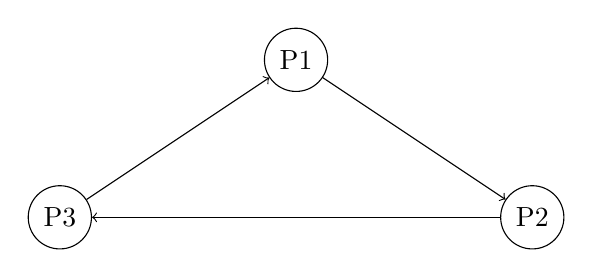
\begin{tikzpicture}

\node[draw,circle] (p1) at (0,2) {P1};
\node[draw,circle] (p2) at (3,0) {P2};
\node[draw,circle] (p3) at (-3,0) {P3};

\draw[->] (p1) -- (p2);
\draw[->] (p2) -- (p3);
\draw[->] (p3) -- (p1);

\end{tikzpicture}
\caption{Circular Wait Condition}
\end{figure}

%====================================================
\section{Resource Allocation Graphs}
%====================================================

\subsection{Definition}

A Resource Allocation Graph (RAG) is a directed graph representing resource ownership and requests.

\subsection{Components}

\begin{itemize}
\item Process = Circle
\item Resource = Rectangle
\end{itemize}

\subsection{Edges}

Request Edge:

\[
P_i \rightarrow R_j
\]

Allocation Edge:

\[
R_j \rightarrow P_i
\]

%----------------------------------------------------
\subsection{Example}
%----------------------------------------------------

\begin{figure}[H]
\centering
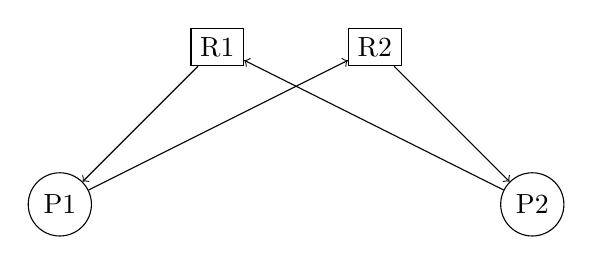
\begin{tikzpicture}

\node[draw,circle] (p1) at (0,0) {P1};
\node[draw,circle] (p2) at (6,0) {P2};

\node[draw,rectangle] (r1) at (2,2) {R1};
\node[draw,rectangle] (r2) at (4,2) {R2};

\draw[->] (r1) -- (p1);
\draw[->] (p1) -- (r2);

\draw[->] (r2) -- (p2);
\draw[->] (p2) -- (r1);

\end{tikzpicture}
\caption{Deadlock in Resource Allocation Graph}
\end{figure}

\subsection{Important Observation}

For systems with a single instance per resource:

Cycle implies deadlock.

%====================================================
\section{Wait-For Graphs}
%====================================================

\subsection{Definition}

A Wait-For Graph removes resource nodes and represents only process dependencies.

\subsection{Construction}

If:

\[
P_i
\]

waits for a resource held by

\[
P_j
\]

draw:

\[
P_i \rightarrow P_j
\]

\subsection{Example}

\begin{figure}[H]
\centering
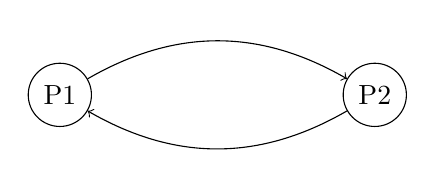
\begin{tikzpicture}

\node[draw,circle] (p1) at (0,0) {P1};
\node[draw,circle] (p2) at (4,0) {P2};

\draw[->] (p1) to[bend left] (p2);
\draw[->] (p2) to[bend left] (p1);

\end{tikzpicture}
\caption{Wait-For Graph Cycle}
\end{figure}

\subsection{Deadlock Rule}

Cycle in WFG implies deadlock.

%====================================================
\section{Deadlock Examples}
%====================================================

\subsection{Example 1: Printer and Scanner}

P1:

\begin{itemize}
\item Holds Printer
\item Requests Scanner
\end{itemize}

P2:

\begin{itemize}
\item Holds Scanner
\item Requests Printer
\end{itemize}

Result:

Deadlock.

%----------------------------------------------------
\subsection{Example 2: Two Mutex Locks}
%----------------------------------------------------

Thread A:

\begin{verbatim}
lock(m1);
lock(m2);
\end{verbatim}

Thread B:

\begin{verbatim}
lock(m2);
lock(m1);
\end{verbatim}

Possible deadlock.

%----------------------------------------------------
\subsection{Example 3: Dining Philosophers}
%----------------------------------------------------

Each philosopher:

\begin{itemize}
\item Holds left fork.
\item Waits for right fork.
\end{itemize}

Deadlock possible.

%====================================================
\section{Deadlocks in Databases}
%====================================================

\subsection{Scenario}

Transaction T1:

\begin{itemize}
\item Locks Row A
\item Requests Row B
\end{itemize}

Transaction T2:

\begin{itemize}
\item Locks Row B
\item Requests Row A
\end{itemize}

Deadlock occurs.

\subsection{Example}

\begin{verbatim}
T1:
LOCK A
LOCK B

T2:
LOCK B
LOCK A
\end{verbatim}

\subsection{Database Handling}

DBMS periodically:

\begin{itemize}
\item Detects deadlocks
\item Rolls back transactions
\end{itemize}

\subsection{Case Study}

MySQL InnoDB:

\begin{itemize}
\item Builds wait-for graph.
\item Detects cycle.
\item Chooses victim transaction.
\item Performs rollback.
\end{itemize}

%====================================================
\section{Deadlocks in Distributed Systems}
%====================================================

\subsection{Challenge}

Resources are distributed across machines.

No global state exists.

\subsection{Examples}

\begin{itemize}
\item Distributed Databases
\item Distributed File Systems
\item Cloud Platforms
\end{itemize}

\subsection{Problem}

Detecting cycles becomes difficult because:

\begin{itemize}
\item Information is distributed.
\item Network delays occur.
\item Partial failures occur.
\end{itemize}

\subsection{Case Study}

Distributed database transaction locks spanning multiple servers.

Global deadlock may involve machines in different data centers.

%====================================================
\section{Deadlocks in Modern Applications}
%====================================================

\subsection{Microservices}

Service A:

\begin{itemize}
\item Calls Service B.
\item Waits for response.
\end{itemize}

Service B:

\begin{itemize}
\item Calls Service A.
\item Waits for response.
\end{itemize}

Distributed deadlock.

\subsection{Cloud Systems}

Examples:

\begin{itemize}
\item Kubernetes controllers
\item Distributed locks
\item Resource schedulers
\end{itemize}

\subsection{Multithreaded Applications}

Common source:

\begin{itemize}
\item Inconsistent lock ordering.
\end{itemize}

%====================================================
\section{Deadlock Detection Concepts}
%====================================================

\subsection{Purpose}

Determine whether deadlock currently exists.

\subsection{Basic Idea}

\begin{itemize}
\item Build dependency graph.
\item Search for cycles.
\end{itemize}

\subsection{For Single Instance Resources}

Use Wait-For Graph.

Cycle indicates deadlock.

\subsection{For Multiple Instances}

Use matrix-based detection algorithms.

\subsection{Detection Frequency}

Tradeoff:

\begin{itemize}
\item Frequent detection = More overhead
\item Infrequent detection = Longer deadlocks
\end{itemize}

\subsection{Deadlock Recovery}

After detection:

\begin{itemize}
\item Kill process
\item Rollback transaction
\item Resource preemption
\end{itemize}

%====================================================
\section{Interview Case Studies}
%====================================================

\subsection{Case Study 1}

Two threads locking resources in opposite order.

Question:

Will deadlock occur?

Answer:

Possible if timing permits.

\subsection{Case Study 2}

A cycle exists in a wait-for graph.

Question:

What does it imply?

Answer:

Deadlock.

\subsection{Case Study 3}

Remove one Coffman condition.

Question:

Can deadlock occur?

Answer:

No.

%====================================================
\section{Key Takeaways}
%====================================================

\begin{itemize}
\item Deadlock is permanent waiting among processes.
\item Resources may be reusable or consumable.
\item Four Coffman conditions are necessary.
\item Mutual exclusion is often unavoidable.
\item Circular wait is easiest to visualize.
\item Resource Allocation Graphs model ownership and requests.
\item Wait-For Graphs simplify deadlock detection.
\item Databases frequently encounter deadlocks.
\item Distributed deadlocks are harder to detect.
\item Deadlock detection relies heavily on cycle detection.
\end{itemize}

%====================================================
\section{20 Interview Questions with Answers}
%====================================================

\begin{enumerate}
\item What is a deadlock?\\
Answer: Permanent waiting among processes due to circular resource dependencies.

\item What are the Coffman conditions?\\
Answer: Mutual exclusion, hold and wait, no preemption, circular wait.

\item Are all four conditions necessary?\\
Answer: Yes.

\item What is mutual exclusion?\\
Answer: Resource cannot be shared simultaneously.

\item What is hold and wait?\\
Answer: Holding resources while requesting others.

\item What is no preemption?\\
Answer: Resources cannot be forcibly removed.

\item What is circular wait?\\
Answer: Circular chain of waiting processes.

\item What is a reusable resource?\\
Answer: Resource used repeatedly after release.

\item Give a reusable resource example.\\
Answer: Printer.

\item What is a consumable resource?\\
Answer: Resource consumed when used.

\item Example of consumable resource?\\
Answer: Message.

\item What is a Resource Allocation Graph?\\
Answer: Graph representing requests and allocations.

\item Process node shape in RAG?\\
Answer: Circle.

\item Resource node shape in RAG?\\
Answer: Rectangle.

\item What is a Wait-For Graph?\\
Answer: Process dependency graph.

\item What does a cycle indicate in WFG?\\
Answer: Deadlock.

\item Why do databases experience deadlocks?\\
Answer: Conflicting locks.

\item What is a deadlock victim?\\
Answer: Process selected for termination/rollback.

\item Why are distributed deadlocks difficult?\\
Answer: No global state.

\item How are deadlocks detected?\\
Answer: Cycle detection.
\end{enumerate}

%====================================================
\section{20 MCQs with Answers}
%====================================================

\begin{enumerate}
\item Deadlock occurs when:
A) CPU idle
B) Infinite waiting
C) Paging
D) Swapping

Answer: B

\item Number of Coffman conditions:
Answer: 4

\item Printer is:
Answer: Reusable Resource

\item Message is:
Answer: Consumable Resource

\item Process nodes in RAG are:
Answer: Circles

\item Resource nodes are:
Answer: Rectangles

\item Circular wait means:
Answer: Circular dependency

\item Hold and wait means:
Answer: Holding while requesting

\item Deadlock requires:
Answer: All four conditions

\item WFG stands for:
Answer: Wait-For Graph

\item Cycle in WFG indicates:
Answer: Deadlock

\item Database deadlock often involves:
Answer: Locks

\item Resource allocation graph contains:
Answer: Processes and Resources

\item Mutual exclusion means:
Answer: Exclusive access

\item No preemption means:
Answer: Cannot forcibly reclaim

\item Distributed deadlock is:
Answer: Harder to detect

\item Detection commonly uses:
Answer: Graph Cycles

\item Recovery may involve:
Answer: Rollback

\item InnoDB can:
Answer: Detect deadlocks

\item Deadlock is a:
Answer: Resource allocation problem
\end{enumerate}

%====================================================
\section{Revision Notes}
%====================================================

\begin{itemize}
\item Deadlock = Permanent waiting.
\item Four Coffman conditions are mandatory.
\item Reusable resources are released after use.
\item Consumable resources disappear after use.
\item RAG contains processes and resources.
\item WFG contains only processes.
\item Cycle in WFG implies deadlock.
\item Databases frequently encounter deadlocks.
\item Distributed deadlocks are challenging.
\item Detection relies on dependency analysis.
\end{itemize}

%====================================================
\section{Cheat Sheet}
%====================================================

\begin{center}
\begin{tabular}{|p{5cm}|p{8cm}|}
\hline
Deadlock & Permanent Waiting \\
\hline
Reusable Resource & Printer, CPU, Memory \\
\hline
Consumable Resource & Message, Signal \\
\hline
Mutual Exclusion & Exclusive Access \\
\hline
Hold and Wait & Hold + Request \\
\hline
No Preemption & Cannot Force Release \\
\hline
Circular Wait & Circular Dependency \\
\hline
RAG & Resource Allocation Graph \\
\hline
WFG & Wait-For Graph \\
\hline
Cycle in WFG & Deadlock \\
\hline
Database Deadlock & Conflicting Locks \\
\hline
Distributed Deadlock & Cross-Machine Dependency \\
\hline
Detection & Cycle Detection \\
\hline
Recovery & Kill / Rollback \\
\hline
\end{tabular}
\end{center}